\documentclass[11pt,a4paper]{article}

\usepackage[T1]{fontenc}
\usepackage{mathptmx}
\usepackage[a4paper,margin=2.5cm]{geometry}
\usepackage{xcolor,graphicx,booktabs,tabularx,array,enumitem,listings,fancyhdr,float}
\usepackage{tikz,pgfgantt}
\usetikzlibrary{positioning,arrows.meta,shapes.geometric,shapes.multipart,fit,calc}
\usepackage[colorlinks=true,linkcolor=black,urlcolor=blue!50!black,citecolor=black]{hyperref}
\usepackage{graphicx}
\usepackage{xcolor}

\newcolumntype{Y}{>{\raggedright\arraybackslash}X}
\newcommand{\st}[1]{\guillemotleft{}#1\guillemotright{}}
\setlist{itemsep=2pt,topsep=4pt}
\renewcommand{\arraystretch}{1.2}

\pagestyle{fancy}
\fancyhf{}
\lhead{\small Shashtho Record -- Project Proposal}
\rhead{\small SEPM Capstone Project }
\cfoot{\small\thepage}

\lstset{
  language=Java,basicstyle=\ttfamily\footnotesize,backgroundcolor=\color{gray!8},
  frame=single,rulecolor=\color{gray!40},breaklines=true,columns=fullflexible,
  keepspaces=true,keywordstyle=\bfseries\color{blue!50!black},commentstyle=\itshape\color{gray},
  numbers=left,numberstyle=\tiny\color{gray},xleftmargin=1.5em
}

\tikzset{
  >=Stealth,
  ext/.style={draw,rectangle,minimum width=2.4cm,minimum height=1cm,align=center,font=\small},
  proc/.style={draw,circle,minimum size=2.1cm,align=center,font=\footnotesize,inner sep=1pt},
  store/.style={draw,rectangle split,rectangle split parts=2,rectangle split horizontal,align=center,font=\footnotesize,rectangle split part fill={gray!20,white}},
  flow/.style={->,thick},
  flowlbl/.style={font=\scriptsize,fill=white,inner sep=1.5pt,align=center,midway},
  act/.style={draw,rounded corners=6pt,minimum width=5.6cm,minimum height=0.8cm,align=center,font=\footnotesize,fill=white},
  dec/.style={draw,diamond,aspect=2.6,inner sep=1pt,font=\footnotesize,align=center,fill=white},
  uc/.style={draw,ellipse,minimum width=3.4cm,minimum height=0.95cm,align=center,font=\footnotesize,fill=white},
  cls/.style={draw,rectangle split,rectangle split parts=3,font=\scriptsize,align=left,text width=4.6cm,inner sep=3pt,fill=white},
  ent/.style={draw,rectangle split,rectangle split parts=2,font=\scriptsize,align=left,inner sep=4pt,fill=white,rectangle split part fill={gray!20,white}},
  obj/.style={draw,rectangle split,rectangle split parts=2,font=\scriptsize,align=left,inner sep=4pt,fill=white,rectangle split part fill={gray!20,white}}
}

\newcommand{\actor}[3]{%
  \draw (#2,#3+0.75) circle (0.2);
  \draw (#2,#3+0.55)--(#2,#3-0.05);
  \draw (#2-0.32,#3+0.4)--(#2+0.32,#3+0.4);
  \draw (#2,#3-0.05)--(#2-0.25,#3-0.6);
  \draw (#2,#3-0.05)--(#2+0.25,#3-0.6);
  \node[below,font=\footnotesize,align=center] at (#2,#3-0.6) {#1};}

\begin{document}

\begin{titlepage}
\centering
\IfFileExists{logo.png}{\includegraphics[width=3.5cm]{logo.png}\\[0.8cm]}{\vspace*{1cm}}
{\large Mawlana Bhashani Science and Technology University\\[2pt]
Department of Information and Communication Technology\par}
\vspace{1.2cm}
% {\large Java Capstone Project 3.1\par}
\vspace{2.2cm}
{\fontsize{30}{36}\selectfont\bfseries Shashtho Record\par}
\vspace{0.4cm}
{\Large A Medical History Tracker with Automatic Antibiotic Labelling\par}

\vspace{0.4cm}
{\itshape For the course of\par}
{\large Software Engineering and Project Management\\
ICT 3107\par}

\vspace{0.6cm}
{\large\textcolor{green!40!black}{Project Proposal and Design Report}\par}
\vspace{0.4cm}
\vfill
% \vspace{5cm}
\begin{tabular}{rl}
\textbf{Submitted by:}  & Ishtiak Ahmed Ayon\\
\textbf{Student ID:}    & IT24039\\
\textbf{Session:}       & 2023-24\\[6pt]
\textbf{Supervisor:}    & Prof. Dr. Ziaur Rahman\\
\textbf{Designation:}   & Professor, Dept. of ICT, MBSTU\\[6pt]
\textbf{GitHub:}        & https://github.com/ishtiakahmedayon/SEPM-Capstone-Project\\

\end{tabular}
\vspace{1cm}
\end{titlepage}

\tableofcontents
\clearpage
% \listoffigures
% \listoftables
\clearpage

\section{Introduction}

\subsection{Background}
Patients visit doctors many times over the years, yet the record of those visits is usually a bundle of paper prescriptions. Symptoms, diagnoses and medicines are forgotten or lost. Knowing which antibiotics were taken, when, and for how long is especially important: repeated or incomplete antibiotic courses contribute to antibiotic resistance, and doctors often ask for this history.

Prescriptions in Bangladesh mostly carry brand names (for example Azithro, Zimax, Ciprocin, Cef-3, Flagyl) rather than generic names. A tracker that only knows generic names cannot recognise most real prescriptions, so the system must hold both generic and local brand names.

\subsection{Problem Statement}
There is no simple, typed, searchable record that links each doctor visit with its symptoms, diagnosis and prescribed medicines, and that automatically shows which medicines are antibiotics.

\subsection{Objectives}
\begin{itemize}
  \item Store each doctor visit with date, doctor, symptoms and diagnosis.
  \item Store the medicines of each visit with dose, frequency and duration.
  \item Label antibiotics automatically on the server using a reference list of generic and Bangladeshi brand names.
  \item List, view, edit, delete and filter visits through a simple, responsive web interface.
  \item Build the system incrementally so that working software exists after every iteration.
\end{itemize}

\subsection{Scope}
\textbf{In scope:} typed data entry, MySQL persistence, server-side validation, antibiotic classification by name matching, Thymeleaf web interface.

\textbf{Out of scope (prototype):} authentication, REST APIs, OCR of prescriptions, AI-based medicine recognition, drug-interaction checking, and any form of medical advice. The antibiotic label is only a name match and is not a clinical decision.

\subsection{Project Summary}
\begin{table}[H]
\centering
\caption{Project summary}
\begin{tabularx}{\textwidth}{lY}
\toprule
\textbf{Item} & \textbf{Detail}\\
\midrule
Project name & Shashtho Record\\
Internal name & \texttt{medtracker} (package and database name)\\
Type & Web application (server-rendered MVC)\\
Language and build & Java 17, Maven\\
Framework & Spring Boot (Web, Data JPA, Validation, Thymeleaf)\\
Database & MySQL, schema \texttt{medtracker}\\
Interface & Plain HTML, one CSS file, minimal inline JavaScript\\
Process model & Iterative and incremental\\
Planned duration & 12 weeks, 5 iterations\\
Repository & [GitHub Repository Link]\\
\bottomrule
\end{tabularx}
\end{table}

\section{Stakeholders, Existing Systems and Feasibility}

\subsection{Stakeholders}
\begin{table}[H]
\centering
\caption{Stakeholders}
\begin{tabularx}{\textwidth}{lYY}
\toprule
\textbf{Stakeholder} & \textbf{Role} & \textbf{Interest}\\
\midrule
Patient / caregiver & Primary user & Keep a clear history of visits and medicines\\
Doctor (indirect) & Reads shared history & Quick view of past diagnoses and antibiotics\\
Developer & Builds and maintains & Clean, extensible design\\
Supervisor & Reviews proposal and progress & Meeting course requirements\\
\bottomrule
\end{tabularx}
\end{table}

\subsection{Existing Approaches}
\begin{table}[H]
\centering
\caption{Comparison with existing approaches}
\begin{tabularx}{\textwidth}{lYYY}
\toprule
\textbf{Approach} & \textbf{Strength} & \textbf{Weakness} & \textbf{Shashtho Record}\\
\midrule
Paper prescriptions & No setup & Lost, unsearchable & Typed and searchable\\
Generic notes apps & Flexible & No structure, no antibiotic flag & Structured visit and medicine data\\
Hospital EMR & Complete & Tied to one hospital, not patient-owned & Patient-owned, local brand names\\
\bottomrule
\end{tabularx}
\end{table}

\subsection{Feasibility Study}
\begin{table}[H]
\centering
\caption{Feasibility summary}
\begin{tabularx}{\textwidth}{lY}
\toprule
\textbf{Type} & \textbf{Assessment}\\
\midrule
Technical & Mature open-source stack; all needed features exist in Spring Boot and MySQL.\\
Economic & No licence cost. Development uses a personal computer and free tools.\\
Operational & Simple forms and tables; no training needed.\\
Schedule & Small scope fits 12 weeks with weekly increments.\\
Legal and ethical & Health data is sensitive. The prototype uses sample data only; encryption and login are future scope.\\
\bottomrule
\end{tabularx}
\end{table}

\section{Requirements}

\subsection{Functional Requirements}
\begin{table}[H]
\centering
\caption{Functional requirements}
\begin{tabularx}{\textwidth}{lY}
\toprule
\textbf{ID} & \textbf{Requirement}\\
\midrule
FR1 & Create a visit with date, doctor, symptoms, diagnosis and at least one named medicine.\\
FR2 & Add and remove medicine rows dynamically on the form.\\
FR3 & Edit an existing visit and its medicines.\\
FR4 & Delete a visit after a confirmation prompt.\\
FR5 & List visits newest first with doctor, diagnosis, medicine count and antibiotic count.\\
FR6 & Filter the list to visits that contain antibiotics.\\
FR7 & Show visit details with a medicine table and an ``Antibiotic'' badge.\\
FR8 & Validate input on the server and show errors inline.\\
FR9 & Set the antibiotic flag on the server only; ignore any client-supplied value.\\
FR10 & Seed the antibiotic reference list at first startup if it is empty.\\
FR11 & Show a 404 page for unknown visit ids.\\
\bottomrule
\end{tabularx}
\end{table}

\subsection{Non-Functional Requirements}
\begin{table}[H]
\centering
\caption{Non-functional requirements}
\begin{tabularx}{\textwidth}{lYY}
\toprule
\textbf{ID} & \textbf{Quality} & \textbf{Requirement}\\
\midrule
NFR1 & Usability & Clean, readable, responsive layout; works on phone and desktop.\\
NFR2 & Performance & List page loads in under one second for up to 1000 visits.\\
NFR3 & Reliability & Visit and medicines are saved in one transaction.\\
NFR4 & Maintainability & Layered packages: controller, service, repository, model, config.\\
NFR5 & Portability & Runs on any OS with Java 17 and MySQL.\\
NFR6 & Data integrity & Antibiotic reference names are unique and lowercase.\\
NFR7 & Security (prototype) & JPA parameterised queries; Thymeleaf output escaping. No login in this version.\\
\bottomrule
\end{tabularx}
\end{table}

\subsection{Assumptions and Constraints}
\begin{itemize}
  \item Single user on a local machine; no concurrent multi-user access.
  \item Antibiotic detection is name matching only (name equals or contains a reference name).
  \item The reference list covers common antibiotics and is not exhaustive.
  \item MySQL 8 is installed and running on port 3306.
\end{itemize}

\section{Software Development Model: Iterative and Incremental}

\subsection{Overview}
The project follows the iterative and incremental model. The system is built in small increments. Each iteration repeats the same cycle (plan, design, build, test, review) and ends with working software that adds to the previous increment. Feedback from each review shapes the next iteration.

\begin{figure}[H]
\centering
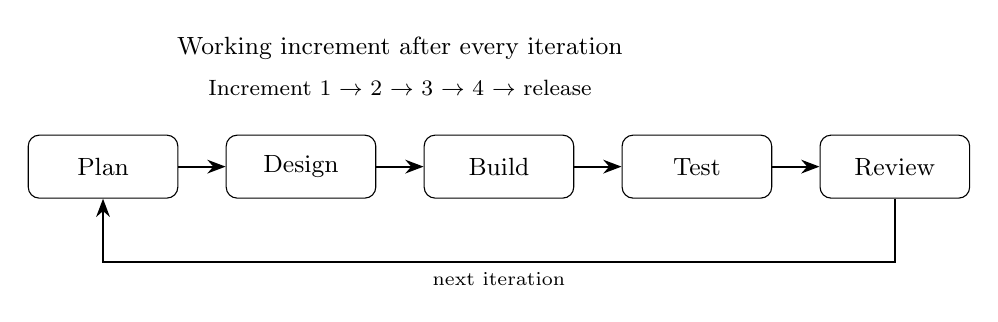
\begin{tikzpicture}[node distance=0.6cm]
  \node[draw,rounded corners=4pt,minimum width=1.9cm,minimum height=0.8cm,font=\small] (pl) {Plan};
  \node[draw,rounded corners=4pt,minimum width=1.9cm,minimum height=0.8cm,font=\small,right=of pl] (de) {Design};
  \node[draw,rounded corners=4pt,minimum width=1.9cm,minimum height=0.8cm,font=\small,right=of de] (bu) {Build};
  \node[draw,rounded corners=4pt,minimum width=1.9cm,minimum height=0.8cm,font=\small,right=of bu] (te) {Test};
  \node[draw,rounded corners=4pt,minimum width=1.9cm,minimum height=0.8cm,font=\small,right=of te] (re) {Review};
  \draw[->,thick] (pl)--(de); \draw[->,thick] (de)--(bu); \draw[->,thick] (bu)--(te); \draw[->,thick] (te)--(re);
  \draw[->,thick] (re.south) -- ++(0,-0.8) -| node[pos=0.25,below,font=\scriptsize]{next iteration} (pl.south);
  \node[font=\small] at ($(de.north)!0.5!(bu.north)+(0,1.1)$) {Working increment after every iteration};
  \node[font=\footnotesize] at ($(de.north)!0.5!(bu.north)+(0,0.6)$) {Increment 1 $\rightarrow$ 2 $\rightarrow$ 3 $\rightarrow$ 4 $\rightarrow$ release};
\end{tikzpicture}
\caption{Iterative and incremental cycle used in Shashtho Record}
\end{figure}

\subsection{Why This Model}
\begin{table}[H]
\centering
\caption{Process model comparison}
\begin{tabularx}{\textwidth}{lYYY}
\toprule
\textbf{Criterion} & \textbf{Waterfall} & \textbf{Iterative and incremental} & \textbf{Fit}\\
\midrule
Requirement changes & Costly & Absorbed each iteration & Medicine rules will evolve\\
Working software & At the end & After every iteration & Early demo to supervisor\\
Risk handling & Found late & Found early & Database and UI risks tested early\\
Documentation & Heavy upfront & Grows with product & Proposal first, refine later\\
\bottomrule
\end{tabularx}
\end{table}

\section{Project Schedule, Milestones and Deliverables}

\subsection{Iteration Plan}
\begin{table}[H]
\centering
\caption{Iteration plan (12 weeks)}
\begin{tabularx}{\textwidth}{llYY}
\toprule
\textbf{Iteration} & \textbf{Weeks} & \textbf{Goals} & \textbf{Increment delivered}\\
\midrule
0 -- Inception & 1--2 & Requirements, feasibility, proposal, UML design & Proposal version 1\\
1 -- Core CRUD & 3--5 & Entities, repositories, MySQL, list, add and detail pages & Visits with medicines can be stored and viewed\\
2 -- Classification & 6--8 & Seeder, normalisation and matching, badge, edit, delete, filter & Antibiotics labelled automatically\\
3 -- Refinement & 9--10 & Validation, 404 page, responsive CSS, testing, feedback fixes & Feature-complete prototype\\
4 -- Release & 11--12 & Final testing, README, report, GitHub release & Final submission\\
\bottomrule
\end{tabularx}
\end{table}

\subsection{Milestones}
\begin{table}[H]
\centering
\caption{Milestones}
\begin{tabularx}{\textwidth}{llYY}
\toprule
\textbf{ID} & \textbf{Week} & \textbf{Milestone} & \textbf{Completion criteria}\\
\midrule
M1 & 2 & Proposal approved & Proposal and UML diagrams reviewed\\
M2 & 5 & Increment 1 & Add, list and detail pages work with MySQL\\
M3 & 8 & Increment 2 & Antibiotic badge, edit, delete and filter work\\
M4 & 10 & Increment 3 & All functional requirements pass tests\\
M5 & 12 & Final submission & Report, code and README on GitHub\\
\bottomrule
\end{tabularx}
\end{table}

\subsection{Deliverables}
\begin{table}[H]
\centering
\caption{Deliverables}
\begin{tabularx}{\textwidth}{llYl}
\toprule
\textbf{ID} & \textbf{Deliverable} & \textbf{Description} & \textbf{Due}\\
\midrule
D1 & Project proposal & This document with UML diagrams & Week 2\\
D2 & Increment 1 & Source code, core CRUD & Week 5\\
D3 & Increment 2 & Source code, classification & Week 8\\
D4 & Increment 3 & Validated, responsive prototype & Week 10\\
D5 & Test results & Manual test case table with results & Week 11\\
D6 & Final package & Source, README, final report, GitHub link & Week 12\\
\bottomrule
\end{tabularx}
\end{table}

\subsection{Resources and Effort}
\begin{table}[H]
\centering
\caption{Resources and effort estimate}
\begin{tabularx}{\textwidth}{lY}
\toprule
\textbf{Resource} & \textbf{Detail}\\
\midrule
Hardware & Personal computer\\
Software & JDK 17, Maven, MySQL 8, MySQL Workbench, IntelliJ IDEA, Git, LaTeX (all free)\\
Effort & About 10 hours per week for 12 weeks, about 120 hours\\
Cost & No monetary cost\\
\bottomrule
\end{tabularx}
\end{table}

\subsection{Gantt Chart}
\begin{figure}[H]
\centering
\resizebox{\textwidth}{!}{%
\begin{ganttchart}[
  hgrid,vgrid={*{1}{draw=gray!40},dotted},
  x unit=0.6cm,y unit title=0.6cm,y unit chart=0.62cm,
  title/.append style={fill=gray!20,draw=gray!50},
  title label font=\footnotesize,
  bar label font=\footnotesize,
  group label font=\footnotesize\bfseries,
  milestone label font=\footnotesize\itshape,
  bar/.append style={fill=blue!45!gray,draw=blue!30!black},
  group/.append style={fill=black!70},
  milestone/.append style={fill=red!70!black},
  bar label node/.append style={align=left},
  group label node/.append style={align=left},
  milestone label node/.append style={align=left}
]{1}{12}
\gantttitle{Week}{12}\\
\gantttitlelist{1,...,12}{1}\\
\ganttgroup{Iteration 0: Inception}{1}{2}\\
\ganttbar{Requirements and feasibility}{1}{1}\\
\ganttbar{Proposal and UML design}{1}{2}\\
\ganttmilestone{M1 Proposal approved}{2}\\
\ganttgroup{Iteration 1: Core CRUD}{3}{5}\\
\ganttbar{Entities, repositories, MySQL}{3}{4}\\
\ganttbar{List, add and detail pages}{4}{5}\\
\ganttmilestone{M2 Increment 1}{5}\\
\ganttgroup{Iteration 2: Classification}{6}{8}\\
\ganttbar{Seeder and matching service}{6}{7}\\
\ganttbar{Edit, delete, filter, badge}{7}{8}\\
\ganttmilestone{M3 Increment 2}{8}\\
\ganttgroup{Iteration 3: Refinement}{9}{10}\\
\ganttbar{Validation, 404, responsive CSS}{9}{10}\\
\ganttbar{Testing and feedback fixes}{9}{10}\\
\ganttmilestone{M4 Increment 3}{10}\\
\ganttgroup{Iteration 4: Release}{11}{12}\\
\ganttbar{Final testing and bug fixes}{11}{11}\\
\ganttbar{Report, README, GitHub release}{11}{12}\\
\ganttmilestone{M5 Final submission}{12}
\end{ganttchart}}
\caption{Project Gantt chart}
\end{figure}

\clearpage
\section{UML and Design Diagrams}

\subsection{Data Flow Diagrams}
Figure~\ref{fig:dfd0} shows the context diagram (Level 0). Figure~\ref{fig:dfd1} decomposes the system into three processes and two data stores (Level 1).

\begin{figure}[H]
\centering
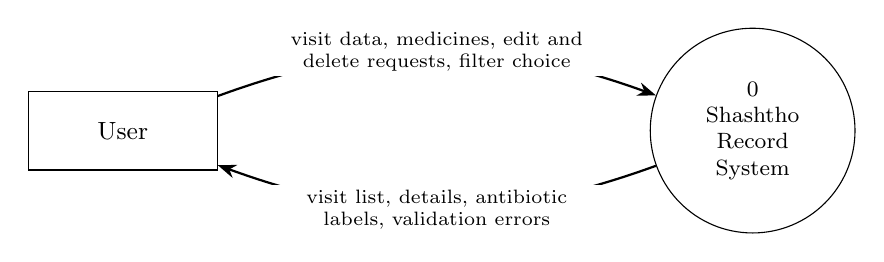
\begin{tikzpicture}
  \node[ext] (user) at (0,0) {User};
  \node[proc,minimum size=2.6cm] (sys) at (8,0) {0\\Shashtho\\Record\\System};
  \draw[flow] (user) to[bend left=20] node[flowlbl,text width=4.2cm]{visit data, medicines, edit and delete requests, filter choice} (sys);
  \draw[flow] (sys) to[bend left=20] node[flowlbl,text width=4.2cm]{visit list, details, antibiotic labels, validation errors} (user);
\end{tikzpicture}
\caption{Data flow diagram, Level 0 (context)}
\label{fig:dfd0}
\end{figure}

\begin{figure}[H]
\centering
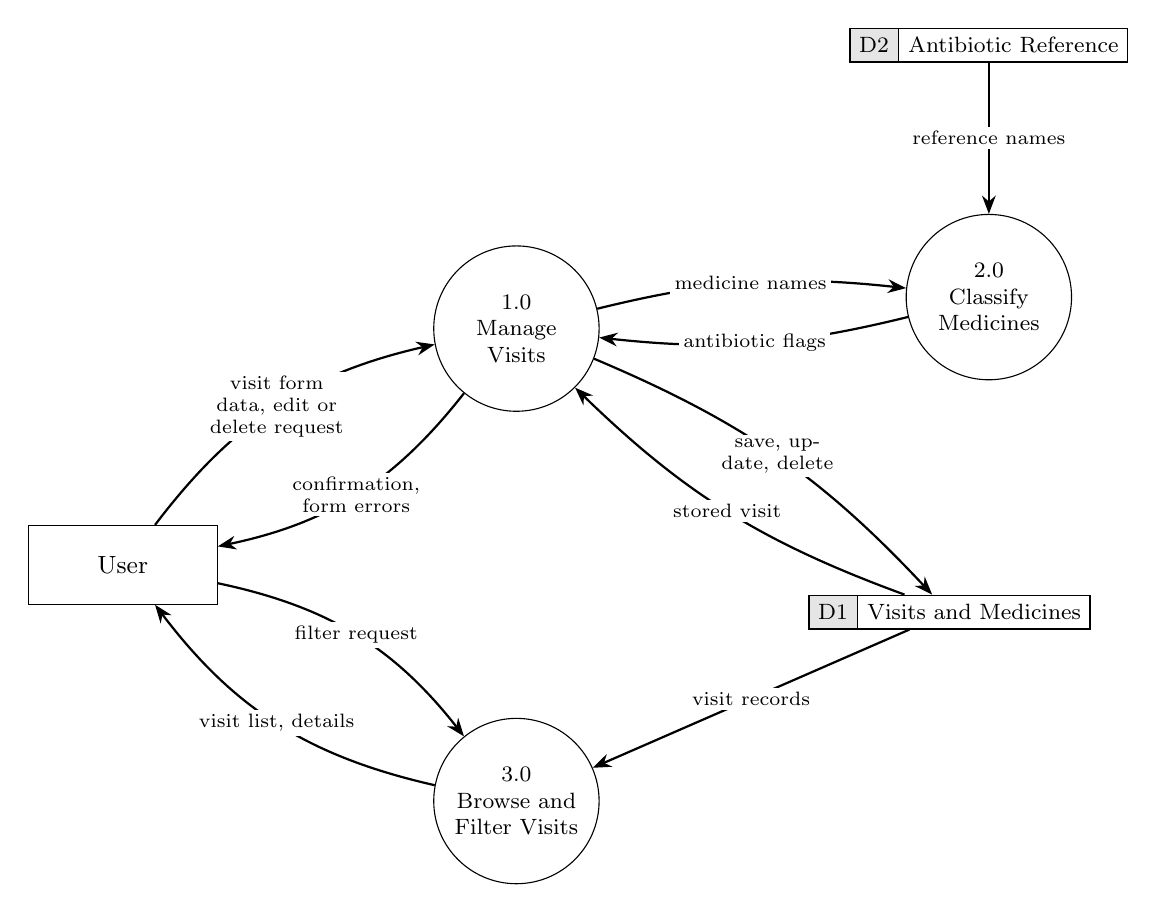
\begin{tikzpicture}
  \node[ext] (user) at (0,0) {User};
  \node[proc] (p1) at (5,3) {1.0\\Manage\\Visits};
  \node[proc] (p2) at (11,3.4) {2.0\\Classify\\Medicines};
  \node[store] (d2) at (11,6.6) {D2\nodepart{two}Antibiotic Reference};
  \node[store] (d1) at (10.5,-0.6) {D1\nodepart{two}Visits and Medicines};
  \node[proc] (p3) at (5,-3) {3.0\\Browse and\\Filter Visits};
  \draw[flow] (user) to[bend left=20] node[flowlbl,text width=2.4cm]{visit form data, edit or delete request} (p1);
  \draw[flow] (p1) to[bend left=20] node[flowlbl,text width=2.2cm]{confirmation, form errors} (user);
  \draw[flow] (p1) to[bend left=10] node[flowlbl]{medicine names} (p2);
  \draw[flow] (p2) to[bend left=10] node[flowlbl]{antibiotic flags} (p1);
  \draw[flow] (d2) -- node[flowlbl]{reference names} (p2);
  \draw[flow] (p1) to[bend left=12] node[flowlbl,text width=2cm]{save, update, delete} (d1);
  \draw[flow] (d1) to[bend left=12] node[flowlbl,text width=1.6cm]{stored visit} (p1);
  \draw[flow] (user) to[bend left=20] node[flowlbl]{filter request} (p3);
  \draw[flow] (p3) to[bend left=20] node[flowlbl,text width=2cm]{visit list, details} (user);
  \draw[flow] (d1) -- node[flowlbl]{visit records} (p3);
\end{tikzpicture}
\caption{Data flow diagram, Level 1}
\label{fig:dfd1}
\end{figure}

\clearpage
\subsection{Use Case Diagram}
\begin{figure}[H]
\centering
\resizebox{\textwidth}{!}{%
\begin{tikzpicture}
  \draw[thick] (4.6,-5.6) rectangle (15.4,5.6);
  \node[font=\small\bfseries] at (10,5.3) {Shashtho Record};
  \actor{User}{1.5}{0}
  \actor{System\\(Data Seeder)}{18.2}{0.2}
  \node[uc] (u1) at (7.6,4.2) {Add Visit};
  \node[uc] (u2) at (7.6,2.6) {Edit Visit};
  \node[uc] (u3) at (7.6,1.0) {Delete Visit};
  \node[uc] (u4) at (7.6,-0.6) {View Visit List};
  \node[uc] (u5) at (7.6,-2.2) {View Visit Details};
  \node[uc] (u6) at (7.6,-3.8) {Filter Antibiotic Visits};
  \node[uc] (u7) at (12.9,4.2) {Validate Input};
  \node[uc] (u8) at (12.9,2.6) {Classify Medicines};
  \node[uc,minimum width=4cm] (u9) at (13.1,0.6) {Seed Antibiotic Reference};
  \foreach \i in {1,...,6} \draw (2.0,0.3) -- (u\i.west);
  \draw (u9.east) -- (17.9,0.6);
  \draw[dashed,->] (u1) -- node[flowlbl,pos=0.75]{\st{include}} (u7);
  \draw[dashed,->] (u2) -- node[flowlbl,pos=0.75]{\st{include}} (u8);
  \draw[dashed,->] (u1) -- node[flowlbl,pos=0.22]{\st{include}} (u8);
  \draw[dashed,->] (u2) -- node[flowlbl,pos=0.22]{\st{include}} (u7);
  \draw[dashed,->] (u6.east) to[out=0,in=0,looseness=1.1] node[flowlbl,pos=0.5]{\st{extend}} (u4.east);
\end{tikzpicture}}
\caption{Use case diagram}
\end{figure}

\begin{table}[H]
\centering
\caption{Use case summary}
\begin{tabularx}{\textwidth}{lYY}
\toprule
\textbf{Use case} & \textbf{Actor} & \textbf{Description}\\
\midrule
Add Visit & User & Enter visit details and medicine rows, then save.\\
Edit Visit & User & Change details or medicines of a saved visit.\\
Delete Visit & User & Remove a visit after confirmation.\\
View Visit List & User & See visits newest first with counts.\\
View Visit Details & User & See one visit with its medicine table and badges.\\
Filter Antibiotic Visits & User & Show only visits that contain antibiotics.\\
Validate Input & System & Check date, doctor and at least one medicine name.\\
Classify Medicines & System & Set the antibiotic flag from the reference list.\\
Seed Antibiotic Reference & Data Seeder & Fill the reference table at first startup.\\
\bottomrule
\end{tabularx}
\end{table}

\clearpage
\subsection{Activity Diagram}
Figure~\ref{fig:act} shows the activity flow for adding a visit.

\begin{figure}[H]
\centering
\resizebox{!}{0.78\textheight}{%
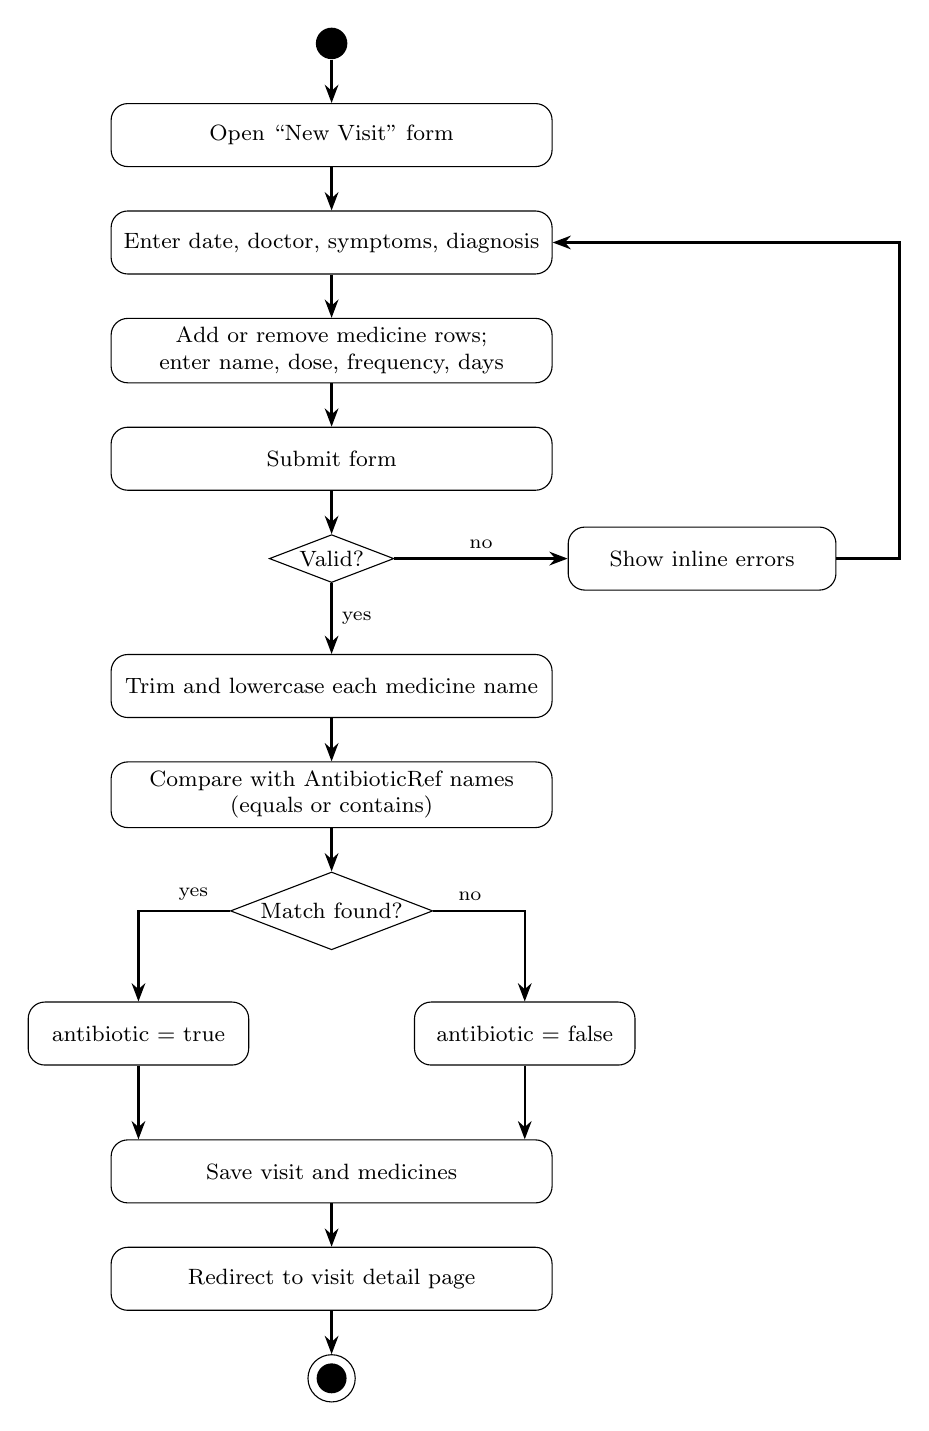
\begin{tikzpicture}[node distance=0.55cm]
  \node[circle,fill=black,minimum size=0.4cm,inner sep=0] (s) {};
  \node[act,below=of s] (a1) {Open ``New Visit'' form};
  \node[act,below=of a1] (a2) {Enter date, doctor, symptoms, diagnosis};
  \node[act,below=of a2] (a3) {Add or remove medicine rows;\\enter name, dose, frequency, days};
  \node[act,below=of a3] (a4) {Submit form};
  \node[dec,below=of a4] (d1) {Valid?};
  \node[act,right=2.2cm of d1,minimum width=3.4cm] (e1) {Show inline errors};
  \node[act,below=0.9cm of d1] (a5) {Trim and lowercase each medicine name};
  \node[act,below=of a5] (a6) {Compare with AntibioticRef names\\(equals or contains)};
  \node[dec,below=of a6] (d2) {Match found?};
  \node[act,below left=0.9cm and 0.4cm of d2,minimum width=2.8cm] (a7) {antibiotic = true};
  \node[act,below right=0.9cm and 0.4cm of d2,minimum width=2.8cm] (a8) {antibiotic = false};
  \node[act,below=2.4cm of d2] (a9) {Save visit and medicines};
  \node[act,below=of a9] (a10) {Redirect to visit detail page};
  \node[circle,draw,minimum size=0.6cm,inner sep=0,below=of a10] (e) {};
  \node[circle,fill=black,minimum size=0.38cm,inner sep=0] at (e) {};
  \draw[flow] (s)--(a1); \draw[flow] (a1)--(a2); \draw[flow] (a2)--(a3); \draw[flow] (a3)--(a4); \draw[flow] (a4)--(d1);
  \draw[flow] (d1) -- node[right,font=\scriptsize]{yes} (a5);
  \draw[flow] (d1) -- node[above,font=\scriptsize]{no} (e1);
  \draw[flow] (e1.east) -- ++(0.8,0) |- (a2.east);
  \draw[flow] (a5)--(a6); \draw[flow] (a6)--(d2);
  \draw[flow] (d2.west) -| node[pos=0.2,above,font=\scriptsize]{yes} (a7.north);
  \draw[flow] (d2.east) -| node[pos=0.2,above,font=\scriptsize]{no} (a8.north);
  \draw[flow] (a7.south) -- (a7.south |- a9.north);
  \draw[flow] (a8.south) -- (a8.south |- a9.north);
  \draw[flow] (a9)--(a10); \draw[flow] (a10)--(e);
\end{tikzpicture}}
\caption{Activity diagram: add a visit}
\label{fig:act}
\end{figure}

\clearpage
\subsection{Entity Relationship Diagram}
\begin{figure}[H]
\centering
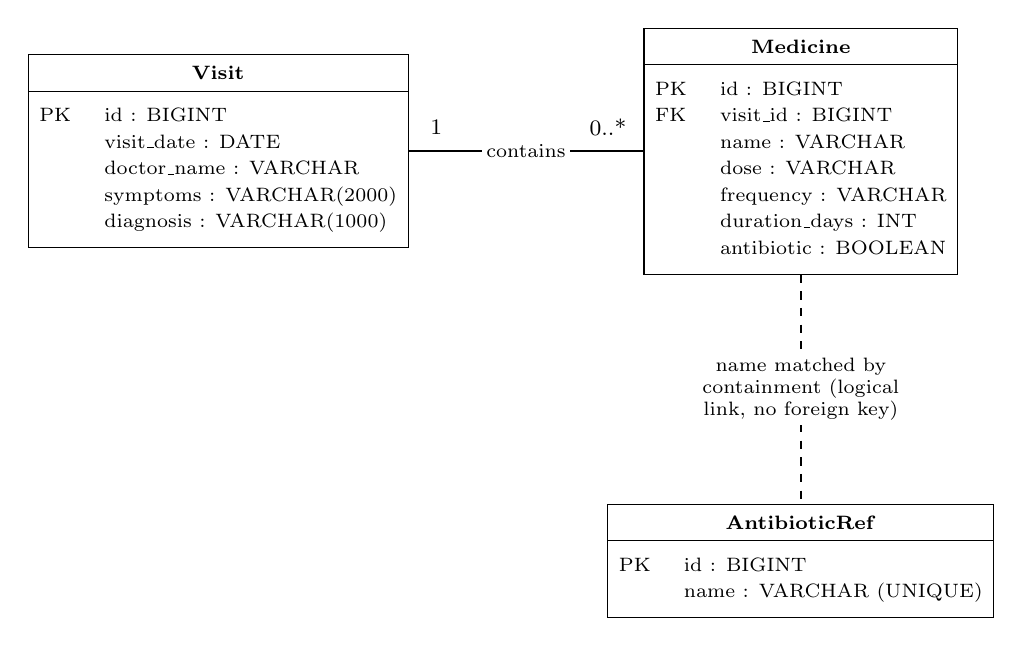
\begin{tikzpicture}
  \node[ent] (visit) at (0,0) {\textbf{Visit}\nodepart{two}\begin{tabular}{@{}ll@{}}
    PK & id : BIGINT\\ & visit\_date : DATE\\ & doctor\_name : VARCHAR\\ & symptoms : VARCHAR(2000)\\ & diagnosis : VARCHAR(1000)\end{tabular}};
  \node[ent] (med) at (7.4,0) {\textbf{Medicine}\nodepart{two}\begin{tabular}{@{}ll@{}}
    PK & id : BIGINT\\ FK & visit\_id : BIGINT\\ & name : VARCHAR\\ & dose : VARCHAR\\ & frequency : VARCHAR\\ & duration\_days : INT\\ & antibiotic : BOOLEAN\end{tabular}};
  \node[ent] (ref) at (7.4,-5.2) {\textbf{AntibioticRef}\nodepart{two}\begin{tabular}{@{}ll@{}}
    PK & id : BIGINT\\ & name : VARCHAR (UNIQUE)\end{tabular}};
  \draw[thick] (visit.east) -- node[flowlbl]{contains} (med.west);
  \node[font=\footnotesize] at ($(visit.east)+(0.35,0.3)$) {1};
  \node[font=\footnotesize] at ($(med.west)+(-0.45,0.3)$) {0..*};
  \draw[thick,dashed] (med.south) -- node[flowlbl,text width=3.6cm]{name matched by containment (logical link, no foreign key)} (ref.north);
\end{tikzpicture}
\caption{Entity relationship diagram}
\end{figure}

\subsection{Class Diagram}
\begin{figure}[H]
\centering
\resizebox{\textwidth}{!}{%
\begin{tikzpicture}
  \node[cls] (ctl) at (0,0) {\centering\textbf{VisitController}\nodepart{second}
    - service : VisitService\nodepart{third}
    + list(antibiotics : boolean) : String\\+ newForm() : String\\+ create(visit) : String\\+ detail(id) : String\\+ editForm(id) : String\\+ update(id, visit) : String\\+ delete(id) : String};
  \node[cls] (exc) at (6,0) {\centering\textbf{VisitNotFoundException}\nodepart{second}
    \st{ResponseStatus} 404\nodepart{third}
    + VisitNotFoundException()};
  \node[cls] (svc) at (0,-5) {\centering\textbf{VisitService}\nodepart{second}
    - visits : VisitRepository\\- antibiotics : AntibioticRefRepository\nodepart{third}
    + list(antibioticsOnly : boolean) : List\\+ get(id : Long) : Visit\\+ create(form : Visit) : Visit\\+ update(id : Long, form : Visit) : Visit\\+ delete(id : Long) : void\\- apply(target, form) : void};
  \node[cls] (seed) at (12,-5) {\centering\textbf{DataSeeder}\nodepart{second}
    - NAMES : List$<$String$>$\\- repository : AntibioticRefRepository\nodepart{third}
    + run(args : String[]) : void};
  \node[cls] (vr) at (0,-9.8) {\centering\st{interface}\\\textbf{VisitRepository}\nodepart{second}
    \nodepart{third}
    + findAllByOrderByVisitDateDescIdDesc() : List\\+ findById(id : Long) : Optional};
  \node[cls] (ar) at (6,-9.8) {\centering\st{interface}\\\textbf{AntibioticRefRepository}\nodepart{second}
    \nodepart{third}
    inherits JpaRepository};
  \node[cls] (visit) at (0,-14.6) {\centering\textbf{Visit}\nodepart{second}
    - id : Long\\- visitDate : LocalDate\\- doctorName : String\\- symptoms : String\\- diagnosis : String\\- medicines : List$<$Medicine$>$\nodepart{third}
    + getAntibioticCount() : long\\+ getters and setters};
  \node[cls] (med) at (6,-14.6) {\centering\textbf{Medicine}\nodepart{second}
    - id : Long\\- name : String\\- dose : String\\- frequency : String\\- durationDays : Integer\\- antibiotic : boolean\nodepart{third}
    + getters and setters};
  \node[cls] (ref) at (12,-14.6) {\centering\textbf{AntibioticRef}\nodepart{second}
    - id : Long\\- name : String\nodepart{third}
    + getName() : String};
  \draw[flow] (ctl) -- node[flowlbl]{uses} (svc);
  \draw[flow,dashed] (svc.north east) -- node[flowlbl]{\st{throws}} (exc.south);
  \draw[flow] (svc) -- node[flowlbl]{uses} (vr);
  \draw[flow] (svc.south east) -- node[flowlbl,pos=0.55]{uses} (ar.north west);
  \draw[flow] (seed.south west) -- node[flowlbl,pos=0.5]{uses} (ar.north east);
  \draw[flow,dashed] (vr) -- node[flowlbl]{\st{manages}} (visit);
  \draw[flow,dashed] (ar.south east) -- node[flowlbl,pos=0.5]{\st{manages}} (ref.north west);
  \draw[{Diamond[length=9pt,width=6pt]}-,thick] (visit.east) -- (med.west);
  \node[font=\scriptsize] at ($(visit.east)+(0.2,0.3)$) {1};
  \node[font=\scriptsize] at ($(med.west)+(-0.35,0.3)$) {0..*};
\end{tikzpicture}}
\caption{Class diagram}
\end{figure}

\clearpage
\subsection{Object Diagram}
Figure~\ref{fig:obj} shows one visit with two medicines at run time. One medicine matches an antibiotic reference name; the other does not.

\begin{figure}[H]
\centering
\begin{tikzpicture}
  \node[obj] (v1) at (4,0) {\underline{v1 : Visit}\nodepart{two}\begin{tabular}{@{}l@{}}id = 1\\visitDate = 2026-10-20\\doctorName = ``Dr. A. Karim''\\symptoms = ``fever, sore throat''\\diagnosis = ``tonsillitis''\end{tabular}};
  \node[obj] (m1) at (0,-5) {\underline{m1 : Medicine}\nodepart{two}\begin{tabular}{@{}l@{}}id = 1\\name = ``Azithro 500''\\dose = ``500 mg''\\frequency = ``1+0+0''\\durationDays = 5\\antibiotic = true\end{tabular}};
  \node[obj] (m2) at (8,-5) {\underline{m2 : Medicine}\nodepart{two}\begin{tabular}{@{}l@{}}id = 2\\name = ``Napa''\\dose = ``500 mg''\\frequency = ``1+1+1''\\durationDays = 3\\antibiotic = false\end{tabular}};
  \node[obj] (r1) at (0,-9.4) {\underline{r1 : AntibioticRef}\nodepart{two}\begin{tabular}{@{}l@{}}id = 7\\name = ``azithro''\end{tabular}};
  \draw[thick] (v1.south) -- ++(0,-0.6) -| node[flowlbl,pos=0.25]{medicines} (m1.north);
  \draw[thick] (v1.south) -- ++(0,-0.6) -| (m2.north);
  \draw[flow,dashed] (m1.south) -- node[flowlbl,text width=3.6cm]{\st{matched by} lowercase name contains ``azithro''} (r1.north);
  \node[font=\scriptsize,text width=3.6cm,align=left] at (8,-9.0) {No reference name is contained in ``napa'', so the flag stays false.};
\end{tikzpicture}
\caption{Object diagram}
\label{fig:obj}
\end{figure}

\section{Implementation}

\subsection{Architecture}
Shashtho Record is a layered Spring Boot MVC application. The controller handles HTTP requests and renders Thymeleaf templates. The service holds business rules and transactions. Repositories access MySQL through Spring Data JPA.

\begin{table}[H]
\centering
\caption{Packages and classes}
\begin{tabularx}{\textwidth}{llY}
\toprule
\textbf{Package} & \textbf{Class} & \textbf{Responsibility}\\
\midrule
controller & VisitController & Routes, form binding, redirect after post\\
service & VisitService & CRUD, normalisation, antibiotic classification\\
service & VisitNotFoundException & Triggers the 404 page\\
repository & VisitRepository & Visit persistence with medicines fetched\\
repository & AntibioticRefRepository & Antibiotic reference persistence\\
model & Visit & Visit entity, validation rules\\
model & Medicine & Medicine entity, antibiotic flag\\
model & AntibioticRef & Reference name entity (unique, lowercase)\\
config & DataSeeder & Seeds reference names when the table is empty\\
\bottomrule
\end{tabularx}
\end{table}
The interface uses all nine classes listed above, which exceeds the minimum of five classes from the class diagram.

\subsection{Classification Rule}
The server ignores any client-supplied antibiotic value. For every medicine row it trims and lowercases the name and sets the flag when the name contains any reference name.

\begin{lstlisting}
String name = m.getName().trim();
String key = name.toLowerCase(Locale.ROOT);
medicine.setAntibiotic(refs.stream().anyMatch(key::contains));
\end{lstlisting}

\subsection{Screens}
\begin{table}[H]
\centering
\caption{Pages}
\begin{tabularx}{\textwidth}{llY}
\toprule
\textbf{Route} & \textbf{Method} & \textbf{Purpose}\\
\midrule
\texttt{/} & GET & Visit list, newest first, with antibiotics-only filter\\
\texttt{/visits/new} & GET & Empty visit form with dynamic medicine rows\\
\texttt{/visits} & POST & Create visit, then redirect\\
\texttt{/visits/\{id\}} & GET & Visit details with medicine table and badges\\
\texttt{/visits/\{id\}/edit} & GET & Edit form\\
\texttt{/visits/\{id\}} & POST & Update visit, then redirect\\
\texttt{/visits/\{id\}/delete} & POST & Delete visit after a confirm prompt\\
\bottomrule
\end{tabularx}
\end{table}

\section{Testing Plan}
\begin{table}[H]
\centering
\caption{Manual test cases}
\begin{tabularx}{\textwidth}{llYY}
\toprule
\textbf{ID} & \textbf{Req.} & \textbf{Test} & \textbf{Expected result}\\
\midrule
T1 & FR1 & Save visit with date, doctor and one medicine & Visit saved, detail page shown\\
T2 & FR8 & Submit with empty doctor & Inline error under doctor field\\
T3 & FR8 & Submit with all medicine names blank & Inline error on medicines\\
T4 & FR2 & Click add and remove medicine row & Rows appear and disappear; at least one row remains\\
T5 & FR9 & Enter ``Zimax 500'' & Antibiotic badge shown\\
T6 & FR9 & Enter ``Napa'' & No badge\\
T7 & FR9 & Tamper the antibiotic field in the request & Value ignored; server result used\\
T8 & FR3 & Edit a visit, remove one medicine & Medicine removed from database\\
T9 & FR4 & Delete and cancel, then delete and confirm & Cancel keeps; confirm removes visit\\
T10 & FR6 & Tick ``Antibiotics only'' & Only visits with antibiotics listed\\
T11 & FR10 & Restart application & Reference list not duplicated\\
T12 & FR11 & Open \texttt{/visits/9999} & 404 page\\
\bottomrule
\end{tabularx}
\end{table}

\section{Risk Management}
\begin{table}[H]
\centering
\caption{Risk register}
\begin{tabularx}{\textwidth}{YllY}
\toprule
\textbf{Risk} & \textbf{Prob.} & \textbf{Impact} & \textbf{Mitigation}\\
\midrule
False antibiotic match from short names & Medium & Medium & Use specific names; review list each iteration\\
Missing brand names in reference list & High & Medium & Seed list is editable data, extended per iteration\\
MySQL setup problems & Medium & High & Documented setup; test database in Iteration 1\\
Schedule slip & Medium & Medium & Fixed scope per increment; drop optional polish first\\
Sensitive health data exposure & Low & High & Sample data only; login and encryption planned\\
\bottomrule
\end{tabularx}
\end{table}

\section{Future Scope}
\begin{itemize}
  \item OCR of prescriptions
  \item AI medicine recognition
  \item Interaction alerts
  \item Login and encryption
  \item Audit log
\end{itemize}

\section{Conclusion}
Shashtho Record gives a simple, structured record of doctor visits and flags antibiotics automatically using generic and local brand names. The iterative and incremental plan delivers a working increment every few weeks, keeps risk low, and leaves a clear path to OCR, AI recognition and security features.

\begin{thebibliography}{9}
\bibitem{som} I. Sommerville, \emph{Software Engineering}, 10th ed., Pearson, 2016.
\bibitem{pre} R. S. Pressman and B. R. Maxim, \emph{Software Engineering: A Practitioner's Approach}, 9th ed., McGraw-Hill, 2019.
\bibitem{fow} M. Fowler, \emph{UML Distilled}, 3rd ed., Addison-Wesley, 2003.
\bibitem{spr} Spring Boot Reference Documentation, \url{https://docs.spring.io/spring-boot/}.
\bibitem{thy} Thymeleaf Documentation, \url{https://www.thymeleaf.org/documentation.html}.
\bibitem{mys} MySQL 8.0 Reference Manual, \url{https://dev.mysql.com/doc/refman/8.0/en/}.
\end{thebibliography}

\end{document}
